\section{Real-Time Scheduler}

The following section describes the preemptive, priority based
scheduler on JOP.

\subsection{Interrupts}

Interrupts are usually associated with low-level programming of
device drivers. The priorities of interrupts and their handler
functions are above task priorities and yield to an immediate context
switch. In this form, interrupts cannot be integrated in a schedule
with \emph{normal} tasks. The execution time of the interrupt handler
has to be integrated in the schedulability analysis as additional
blocking time. A better solution is to handle interrupts, which
represent external events, as schedulable objects with priority
levels in the range of real-time tasks, as suggested in the RTSJ.

\paragraph{The Timer Interrupt}

The timer or clock interrupt has a different semantic than other
interrupts. The main purpose of the timer interrupt is representation
of time and release of periodic or time triggered tasks. One common
implementation is a clock tick. The interrupt occurs at a regular
interval (e.g.\ 10 ms) and a decision has to be taken whether a task
has to be released. This approach is simple to implement, but there
are two major drawbacks: The resolution of timed events is bound by
the resolution of the clock tick and clock ticks without a task
switch are a waste of execution time.

A better approach, used in JOP, is to generate timer interrupts at
the release times of the tasks. The scheduler is now responsible for
reprogramming the timer after each occurrence of a timer interrupt.
The list of sleeping threads has to be searched to find the nearest
release time in the future of a higher priority thread than the one
that will be released now. This time is used for the next timer
interrupt.

\paragraph{External Events}

Hardware interrupts, other than the timer interrupt, are represented
as instances of \code{Runnable}. The interrupt handler runs at top
priority. To incorporate external event handling as a \emph{normal}
schedulable object under the control of the scheduler the interrupt
handler can simply fire software event. In that case the handler code
executes in the associated thread. When the minimum interarrival time
of the hardware events is known, these events can be incorporated
into the priority assignment and schedulability analysis in the same
way as periodic tasks.

\paragraph{Software Interrupts}

The common software generated interrupts, such as illegal memory
access or divide by zero, are represented by Java runtime exceptions
and need no special handler. They can be detected with a try-catch
block.

Asynchronous notification from the program is supported, in the same
way as an external event, as a schedulable object with an associated
thread. The event is triggered through the call of \code{fire()}. The
thread with the handler is placed in the runnable state and scheduled
according to its priority.


\subsection{Task Switch}

An important issue in real-time systems is the time for a task
switch. A task switch consists of two actions:
\begin{itemize}
    \item \emph{Scheduling} is the selection of the task order
        and timing
    \item \emph{Dispatching} is the term for the context switch
        between tasks
\end{itemize}

\paragraph{Scheduling}

Most real-time systems use a fixed-priority preemptive scheduler.
Tasks with the same priority are usually scheduled in a FIFO order.
Two common ways to assign priorities are rate monotonic or, in a more
general form, deadline monotonic assignment. When two tasks get the
same priority, we can choose one of them and assign a higher priority
to that task and the task set is still schedulable. We get a strictly
monotonic priority order and do not have to deal with FIFO order.
This eliminates queues for each priority level and results in a
single, priority ordered task list.

Strictly fixed priority schedulers suffer from a problem called
\emph{priority inversion} \cite{626613}. The problem where a low
priority task blocks a high priority task on a shared resource is
solved by raising the priority of the low priority task. Two standard
priority inversion avoidance protocols are common:
%
\begin{description}
    \item[Priority Inheritance Protocol:] A lock assigns the
        priority of the highest-priority waiting task to the task
        holding the lock until that task releases the resource.

    \item[Priority Ceiling Emulation Protocol:] A lock gets a
        priority assigned above the priority of the
        highest-priority task that will ever acquire the lock.
        Every task will be immediately assigned the priority of
        that lock when acquiring it.
\end{description}
%
The priority inheritance protocol is more complex to implement and
the time when the priority of a task is raised is not so obvious. It
is not raised because the task does anything, but because another
task reaches some point in its execution path.

Using priority ceiling emulation with unique priorities, different
from task priorities, the priority order is still strictly monotonic.
The priority ordered task list is expanded with slots for each lock.
If a task acquires a lock, it is placed in the corresponding slot.
With this extension to the task list, scheduling is still simple and
can be efficiently implemented.

In the current implementation of JOP locks have implicitly top
priority. On a uniprocessor system this top priority is enforced by
switching off the interrupts. In the CMP version of JOP a single
global lock is acquired at \code{monitorenter}. 

\paragraph{Dispatching}


The time for a context switch depends on the size of the state of the
tasks. For a stack machine it is not so obvious what belongs to the
state of a task. If the stack resides in main memory, only a few
registers (e.g. program counter and stack pointer) need to be saved
and restored. However, the stack is a frequently accessed memory
region of the JVM. The stack can be seen as a data cache and should
be placed near the execution unit (in this case, \emph{near} means on
the chip and not in external memory). However, on-chip memory is
usually too small to hold the stack content for all tasks. This means
that the stack is part of the execution context and has to be saved
and restored on a context switch.

In JOP, the stack is placed in local (on-chip) FPGA memory with
single cycle access time. With this configuration, the next question
is how much of the stack to place there. Either the complete stack of
a thread or only the stack frame of the current method can reside
locally. If the complete stack of a thread is stored in local memory,
the invocation of methods and returns are fast, but the context is
large. For fast context switches, it is preferable to have only a
short stack in local memory. This results in less data being
transferred to and from main memory, but more memory transfers on
method invocation and return. The local stack can be further divided
into small pieces, each holding only one stack frame of one thread.
During the context switch, only the stack pointer needs to be saved
and restored. The outcome of this is a very fast context switch,
although the size of the local memory limits the maximum number of
threads.

Since JOP is a soft-core processor, these different solutions can be
configured for different application requirements. It is even
possible to mix of these policies: some stack slots can be assigned
to \emph{important} threads, while the remaining threads share one
slot. This stack slot only needs to be exchanged with the main memory
when switching \emph{to} a less \emph{important} thread.


\section{User-Defined Scheduler}
\label{sec:usersched}

The novel approach to implement a real-time scheduler in Java opens
up new possibilities. An obvious next step is to extend this system
to provide a framework for user-defined scheduling in Java. New
applications, such as multimedia streaming, result in \emph{soft}
real-time systems that need a more flexible scheduler than the
traditional fixed priority based ones. This section provides a
simple-to-use framework to evaluate new scheduling concepts for
these applications in real-time Java.

The following section analyzes which events are exposed to the
scheduler and which functions from the JVM need to be available in
the user space. It is followed by the definition of the framework
and examples of how to implement a scheduler using this framework.

\subsection{Schedule Events}

The most important element of the user-defined scheduler is to
define which events result in the scheduling of a new task. When
such an event occurs, the user-defined scheduler is invoked. It can
update its task list and decide which task is dispatched.

\begin{description}

\item[Timer interrupt:] For timed scheduling decisions, a programmable
timer generates exact timed interrupts. The scheduler controls the
time interval for the next interrupt.

\item[HW interrupt:] Each hardware-generated interrupt can be associated
with an asynchronous event. This allows the execution of a device
driver under the control of the scheduler. Latencies of the device
driver can be controlled by assigning the right priority in a
priority scheduler.

\item[Monitor:] To allow different implementations of priority inversion
protocols, hooks for \code{monitorenter} and \code{monitorexit} are
provided.

\item[Thread block:] Each thread can cease execution via a call of the
scheduler. This function is used to implement methods such as
\code{waitForNextPeriod()} or \code{sleep()}. The reason for
blocking (e.g. end of periodic work) has to be communicated to the
scheduler (e.g. next time to be unblocked for a periodic task).

\item[SW event:] Invoking \code{fire()} on an event provides support for
signaling. \code{wait()}, \code{notify()} or \code{notifyAll()} are
not necessary. However, this mechanism is not part of the scheduling
framework. It can be implemented with the user-defined scheduler and
an associated thread class.

\end{description}

\subsection{Data Structures}

To implement a scheduler in Java, some internal JVM data structures
need to be accessible.

\begin{description}

\item[Object:] In Java, any object (including an object from the class
\code{Class} for static methods) can be used for synchronization.
Different priority inversion protocols require different data
structures to be associated with an object. Each object provides a
field, accessed through a \code{Scheduler} method, in which these
data structures can be attached.

\item[Thread:] A list of all threads is provided to the scheduler. The
scheduler is also notified when a new thread object is created or a
thread terminates. The scheduler controls the start of threads.

\end{description}

\subsection{Services for the Scheduler}

The real-time JVM and the hardware platform have to provide some
minimum services. These services are exposed through
\code{Scheduler}:

\begin{description}

\item[Dispatch:] The current active thread is interrupted and a new
thread is placed in the run state.

\item[Time:] System time with high resolution (microseconds, if the
hardware can provide it) is used for time derived scheduling
decisions.

\item[Timer:] A programmable timer interrupt (not a timer tick) is
necessary for accurate time triggered scheduling.

\item[Interrupts:] To protect the data structures of the scheduler all
interrupts can be disabled and enabled.

\end{description}

\subsection{Class Scheduler}

The class \code{Scheduler} has to be extended to implement a
user-defined scheduler. The class \code{Task} represents
\emph{schedulable objects}. For non-trivial scheduling algorithms,
\code{Task} is also extended. The scheduler lives in normal thread
space. There is no special context such as kernel space. The methods
of \code{Scheduler} are categorized by the caller module and
described in detail below.

\paragraph{Application}

To use a scheduler in an application, the application only has to
create one instance of the scheduler class and has to decide when
scheduling starts.

\begin{lstlisting}[emph=Scheduler]
public Scheduler()
\end{lstlisting}
A single instance of the scheduler is created by the application.

\begin{lstlisting}[emph=start]
public void start()
\end{lstlisting}
This method initiates the transition to the mission phase of the
application. All created tasks are started and scheduled under the
control of the user scheduler.

\paragraph{Task}

A user-defined scheduler usually needs an associated user-defined
thread class (an extension of \code{Task}). This class interacts
with the scheduler by invoking following methods from
\code{Scheduler}:

\begin{lstlisting}[emph=addTask]
void addTask(Task t)
\end{lstlisting}
The scheduler has access to the list of created tasks to use at the
start of scheduling. For dynamic task creation after the start of
the scheduler, this method is called by the constructor of Task, to
notify the scheduler to update its list.

\begin{lstlisting}[emph=isDead]
void isDead(Task t)
\end{lstlisting}
The scheduler is notified when a Task returns from the \code{run()}
method. The scheduler removes this Task from the list of schedulable
objects.

\begin{lstlisting}[emph=block]
void block()
\end{lstlisting}
Every \code{Task} can cease execution via a call of the scheduler.
This method is used to implement methods such as
\code{waitForNextPeriod()} or \code{sleep()} in a user defined
thread class.

\paragraph{Java Virtual Machine}

The methods listed below provide the essential points of
communication between the JVM and the scheduler. As a response to an
interrupt (hardware or timer), entrance or exit of a synchronized
method/block the JVM invokes a method from the scheduler.

\begin{lstlisting}[emph=schedule]
abstract void schedule()
\end{lstlisting}
This is the main entry point for the scheduler. This method has to
be overridden to implement the scheduling algorithm. It is called
from the JVM on a timed event or a software interrupt (see
\code{genInt()}) is issued (e.g. when a \code{Task} gives up
execution).

\begin{lstlisting}[emph=interrupt]
void interrupt(int nr)
\end{lstlisting}
The scheduler is notified on a hardware event. It can directly call
an associated device driver or use this information to unblock a
waiting task.

\begin{lstlisting}[emph={monitorEnter,monitorExit}]
 void monitorEnter(Object o)
 void monitorExit(Object o)
\end{lstlisting}
These methods are invoked by the JVM on synchronized methods and
blocks (JVM bytecodes \code{monitorenter} and \code{monitorexit}).
They provide hooks for executing dynamic priority changes in the
scheduler.

\paragraph{Scheduler}

Services of the JVM needed to implement a scheduler are provided
through static methods.

\begin{lstlisting}[emph=genInt]
static final void genInt()
\end{lstlisting}
This service from the JVM schedules a software interrupt. As a
result, \code{schedule()} is called. This method is the standard way
of switching control to the scheduler. It is e.g. invoked by
\code{block()}.

\begin{lstlisting}[emph={enableInt,disableInt}]
 static final void enableInt()
 static final void disableInt()
\end{lstlisting}
The scheduler cannot use monitors to protect its data structures as
the scheduler itself is in charge of handling monitors. To protect
the data structures of the scheduler, it can globally enable and
disable interrupts.

\begin{lstlisting}[emph=dispatch]
static final void dispatch(Task nextTask, int nextTim)
\end{lstlisting}
This method dispatches a \code{Task} and schedules a timer interrupt
at \code{nextTim}.

\begin{lstlisting}[emph={attachData,getAttachedData}]
 static final void attachData(Object obj, Object data)
 static final Object getAttachedData(Object obj)
\end{lstlisting}
The behavior of the priority inversion avoidance protocol is defined
by the user scheduler. The root of the Java class hierarchy
(\code{java.lang.Object}) contains a JVM internal reference of
generic type Object that can be used by the scheduler to attach data
structures for monitors. The first argument of these methods is the
object to be used as a monitor.

\paragraph{Scheduler or Task}

The following two methods are utility functions useful for the
scheduler and the thread implementation.

\begin{lstlisting}[emph=getNow]
static final int getNow()
\end{lstlisting}
To support time-triggered scheduling, the system provides access to
a high-resolution time or counter. The returned value is the time
since startup in microseconds. The exact resolution is
implementation-dependent.

\begin{lstlisting}[emph=getRunningTask]
static final Task getRunningTask()
\end{lstlisting}
The current running \code{Task} (in which context the scheduler is
called) is returned by this method.

\subsection{Class Task}

A basic structure for schedulable objects is shown in
Listing~\ref{lst:arch:rt:user:task}. This class is usually extended
to provide a thread implementation that fits in the user-defined
scheduler. The class \code{Task} is intended to be minimal. To avoid
inheriting methods that do not fit for some applications, it does not
extend \code{java.lang.Thread}. However, \code{Task} can be used to
\emph{implement} \code{java.lang.Thread}.

\begin{lstlisting}[float,caption=A basic schedulable object,
label=lst:arch:rt:user:task, emph={Task, start, enterMemory,
exitMemory,run,getFirstTask,getNextTask}]
    public class Task {

        public Task()
        public Task(Memory mem)
        void start()

        public void enterMemory()
        public void exitMemory()

        public void run()

        static Task getFirstTask()
        static Task getNextTask()
    }
\end{lstlisting}

The methods \code{enterMemory} and \code{exitMemory} are used by the
application to provide scoped memory for temporary allocated
objects. \code{Task} provides a list of active tasks for the
scheduler.

One issue, raised by the implementation of the framework, is the way
in which access rights to methods need to be defined in Java. All
methods, except \code{start()}, should be \code{private} or
\code{protected}. However, some methods, such as \code{schedule()},
are invoked by a part of the JVM, which is also written in Java but
resides in a different package. This results in defining the methods
as public and \emph{hoping} that they are not invoked by the
application code. The C++ concept of friends would greatly help in
sharing information over package boundaries without making this
information public.

\subsection{A Simple Example Scheduler}

Listing~\ref{lst:arch:rt:user:example} shows a full example of using
this framework to implement a simple round robin scheduler.

The only method that needs to be supplied is \code{schedule()}. For
a more advanced scheduler, it is necessary to provide a combination
of a user defined thread class and a scheduler class. These two
classes have to be tightly integrated, as the scheduler uses
information provided by the thread objects for its scheduling
decisions.

\pagebreak
\begin{lstlisting}[caption=A very simple scheduler,
label=lst:arch:rt:user:example]
    public class RoundRobin extends Scheduler {

        //
        //   test threads
        //
        static class Work extends Task {

            private int c;

            Work(int ch) {
                c = ch;
            }

            public void run() {

                for (;;) {
                    Dbg.wr(c); // debug output

                    // busy wait to simulate
                    // 3 ms workload in Work.
                    int ts = Scheduler.getNow();
                    ts += 3000;
                    while (ts-Scheduler.getNow()>0)
                        ;
                }
            }
        }

        //
        //    user scheduler starts here
        //

        public void addTask(Task t) {
            // we do not allow tasks to be
            // added after start().
        }

        //
        //    called by the JVM
        //
        public void schedule() {
            Task t = getRunningTask().getNextTask();
            if (t==null) t = Task.getFirstTask();
            dispatch(t, getNow()+10000);
        }


        public static void main(String[] args) {

            new Work('a');
            new Work('b');
            new Work('c');

            RoundRobin rr = new RoundRobin();

            rr.start();
        }
    }
\end{lstlisting}


\subsection{Interaction of Task, Scheduler and the JVM}

The framework is used to re-implement the scheduler described in
Section~\ref{sec:rtprof}. In the original implementation, the
interaction between scheduling and threads was simple, as the
scheduling was part of the thread class. Using the framework, these
functions have to be split to two classes, extending \code{Task} and
\code{Scheduler}. Both classes are placed in the same package to
provide simpler information sharing with some protection from the
rest of the application. For performance reasons, data structures are
directly exposed from one class to the other.

The resulting implementation is compatible with the first
definition, with the exception that \code{RtThread} now extends
\code{Task}. However, no changes in the application code are
necessary.

\figurename~\ref{fig_arch_rt_user_interaction} is an interaction
example of this scheduler within the framework. The interaction
diagram shows the message sequences between two application tasks,
the scheduler, the JVM and the hardware. The hardware represents
interrupt and timer logic. The corresponding code fragments of the
application, \code{RtThread} and \code{PriorityScheduler} are shown
in Listing~\ref{lst:arch:rt:user:app}, \ref{lst:arch:rt:user:rtthr}
and \ref{lst:arch:rt:user:prsched}. Task 2 is a periodic task with a
higher priority than Task 1.

\begin{figure*}
    \centering
    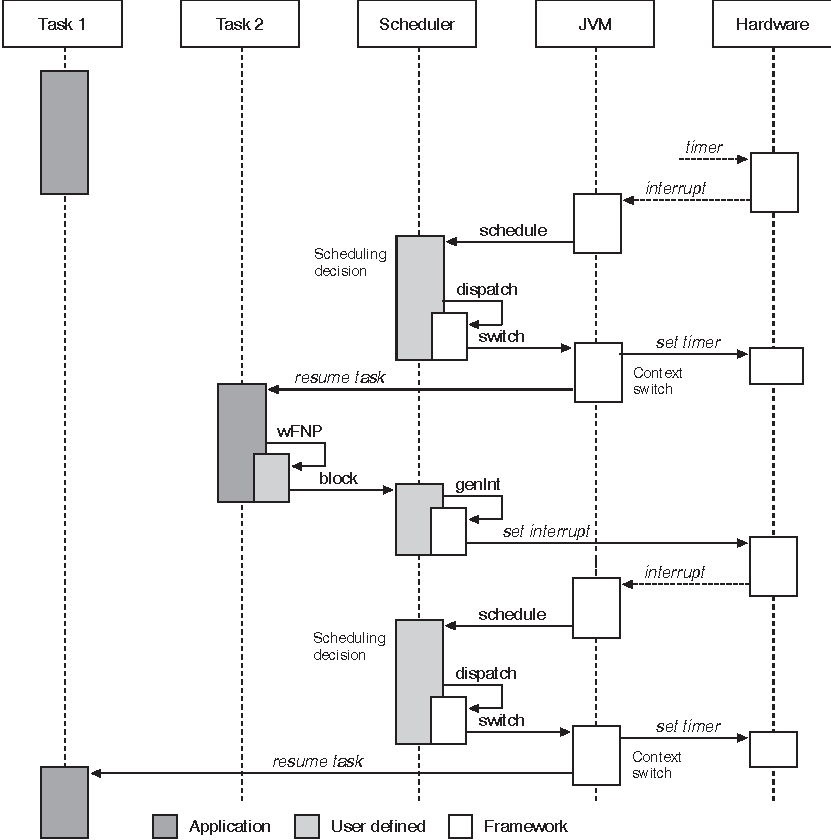
\includegraphics[scale=\picscale]{runtime/rt_user_interaction}
    \caption[Interaction diagram of the user scheduler framework]
    {Interaction and message exchange between the application,
the scheduler, the JVM and the hardware}
    \label{fig_arch_rt_user_interaction}
\end{figure*}

The first event is a timer event to unblock Task 2 for a new period.
The generated timer event results in a call of the user defined
scheduler. The scheduler performs its scheduling decision and issues
a context switch to Task 2. With every context switch the timer is
reprogrammed to generate an interrupt at the next time triggered
event for a higher priority task. Task 2 performs the periodic work
and ceases execution by invocation of \code{waitForNextPeriod()}.
The scheduler is called and requests an interrupt from the hardware
resulting in the same call sequence as with a timer or other
hardware interrupt. The software generated interrupt imposes
negligible overhead and results in a single entry point for the
scheduler. Task 1 is the only ready task in this example and is
resumed by the scheduler.

Using a general scheduling framework for a real-time scheduler is
not without its costs. Additional methods are invoked from a
scheduling event until the actual dispatch takes place. The context
switch is about 20\% slower than in the original implementation. It
is the opinion of the author that the additional cost is outweighed
by the flexibility of the framework.

\begin{lstlisting}[float,caption={Code fragment oft the application},
label=lst:arch:rt:user:app]
        for (;;) {
            doPeriodicWork();
            waitForNextPeriod();
        }
\end{lstlisting}

\begin{lstlisting}[float,caption={Implementation in RtThread},
label=lst:arch:rt:user:rtthr]
    public boolean waitForNextPeriod() {

        synchronized(monitor) {

            // ps is the instance of
            // the PriorityScheduler
            int nxt = ps.next[nr] + period;

            int now = Scheduler.getNow()
            if (nxt-now < 0) {
                // missed deadline
                doMissAction();
                return false;
            } else {
                // time for the next unblock
                ps.next[nr] = nxt;
            }
            // just schedule an interrupt
            // schedule() gets called.
            ps.block();
        }
        return true;
    }
\end{lstlisting}

\begin{lstlisting}[float,caption={Implementation of the PriorityScheduler},
label=lst:arch:rt:user:prsched]
    public void schedule() {

        // Find the ready thread with
        // the highest priority.
        int nr = getReady();

        // Search the list of sleeping threads
        // to find the nearest release time
        // in the future of a higher priority
        // thread than the one that will be
        // released now.
        int time = getNextTimer(nr);

        // This time is used for the next
        // timer interrupt.
        // Perform the context switch.
        dispatch(task[nr], time);
        // No access to locals after this point.
        // We are running in the NEW context!
    }
\end{lstlisting}


\subsection{Predictability}

The architecture of JOP is designed to simplify WCET analysis. Every
JVM bytecode maps to one ore more microcode instructions. Every
microcode instruction takes exactly one cycle to execute. Thus, the
execution time at the bytecode level is known cycle accurately. The
microcode contains no data dependent or unbound loops that would
compromise the WCET analysis (see Chapter~\ref{chap:wcet}).

The worst-case time for dispatching is known cycle accurately on
this architecture. Only the time behavior of the user scheduler
needs to be analyzed. With the known WCET of every bytecode, as
listed in Appendix~\ref{appx:bytecode}, the WCET of the scheduler
can be obtained by examining it at the bytecode level. This can be
done manually or with a WCET analysis tool.

\subsection{Related Work}

Several implementations of user-level schedulers in standard
operating systems have been proposed. In \cite{REDLinux2003}, the
Linux scheduling mechanism is enhanced. It is divided into a
dispatcher and an allocator. The dispatcher remains in kernel space;
while the allocator is implemented as a user space function. The
allocator transforms four basic scheduling parameters (priority,
start time, finish time and budget) into scheduling attributes to be
used by the dispatcher. Many existing schedulers can be supported
with this parameter set, but others that are based on different
parameters cannot be implemented. This solution does not address the
implementation of protocols for shared resources.

A different approach defines a new API to enable applications to use
application-defined scheduling in a way compatible with the
scheduling model defined in POSIX \cite{787339}. It is implemented
in the MaRTE OS, a minimal real-time kernel that provides the C and
Ada language POSIX interface. This interface has been submitted to
the Real-Time POSIX Working Group for consideration.

One approach to user-level scheduling in Java can be found in
\cite{Feizabadi:2003:UAS}. A thread \emph{multiplexor}, as part of
the FLEX ahead-of-time compiler system for Java, is used for utility
accrual scheduling. However, the underlying operating system -- in
this case Linux -- can still be seen through the framework and there
is no support for Java synchronization.

\subsection{Summary}

This section and Section~\ref{sec:rtprof} consider the
implementation of real-time scheduling on a Java processor. The
novelty of the described approach is in implementing functions
usually associated with an RTOS in Java. That means that real-time
Java is not based on an RTOS, and therefore not restricted to the
functionality provided by the RTOS. With JOP, a self-contained
real-time system in pure Java becomes possible. This system is
augmented with a framework to provide scheduling functions at the
application level. The implementation of the specification,
described in Section~\ref{sec:rtprof}, is successfully used as the
basis for a commercial real-time application in the railway
industry. Future work will extend this framework to support multiple
schedulers. A useful combination of schedulers would be: one for
standard \code{java.lang.Thread} (optimized for throughput), one for
soft real-time tasks and one for hard real-time tasks.
